\documentclass[grid,avery5371]{flashcards}

\usepackage[utf8]{inputenc}
\usepackage[T1]{fontenc}
\usepackage{verse}
\usepackage[version=3]{mhchem}
\usepackage{graphicx}
\settowidth{\versewidth}{It lies behind stars and under hills,}
\addtolength{\versewidth}{2em}

\geometry{headheight=12pt}
\usepackage{fancyhdr}
\pagestyle{fancy}
\fancyhf{}
\renewcommand{\headrulewidth}{0pt}


\title{Conversion flashcards}
\author{Sam Robbins}

\cardbackstyle[\LARGE\bfseries]{plain}
\cardfrontstyle[\large]{headings}


\begin{document}

\begin{flashcard}[1eV=]{%
\begin{verse}[\versewidth]
\Huge{$1.6\times10^{-19}$J}
\end{verse}}
1eV in J
\end{flashcard}

\begin{flashcard}[1kWh=]{%
\begin{verse}[\versewidth]
\Huge{$3.6\times10^{6}$J}
\end{verse}}
1kWh in J
\end{flashcard}

\begin{flashcard}[Alpha Decay]{%
\begin{verse}[\versewidth]
\Huge{\ce{^{\normalsize{A}}_{\normalsize{Z}}X}$\rightarrow$\ce{^{\normalsize{A-4}}_{\normalsize{Z-2}}X}+\ce{^{\normalsize{4}}_{\normalsize{2}}He}}
\end{verse}}
Alpha decay
\end{flashcard}

\begin{flashcard}[Beta$^-$ decay]{%
\begin{verse}[\versewidth]
\Huge{\ce{^{\normalsize{A}}_{\normalsize{Z}}X}$\rightarrow$\ce{^{\normalsize{A}}_{\normalsize{Z+1}}X}+$e^-$+$\nu^-$}
\end{verse}}
Beta$^-$ decay
\end{flashcard}

\begin{flashcard}[]{%
\begin{verse}[\versewidth]
\Huge{Diode}
\end{verse}}
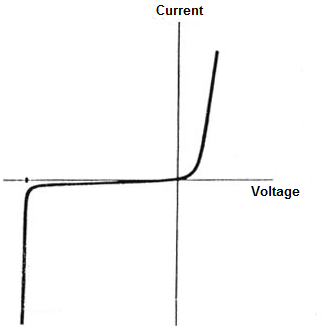
\includegraphics[width=4.5cm, height=4.5cm]{Diode.png}
\end{flashcard}

\begin{flashcard}[]{%
\begin{verse}[\versewidth]
\Huge{Resistor}
\end{verse}}
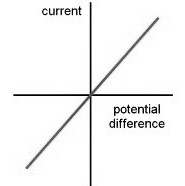
\includegraphics[width=4.5cm, height=4.5cm]{Resistor.jpg}
\end{flashcard}

\begin{flashcard}[]{%
\begin{verse}[\versewidth]
\Huge{Bulb}
\end{verse}}
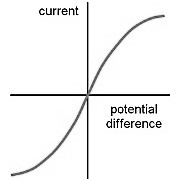
\includegraphics[width=4.5cm, height=4.5cm]{Bulb.jpg}
\end{flashcard}

\begin{flashcard}[]{%
\Huge{Thermistor}}
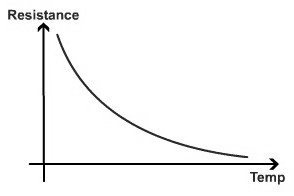
\includegraphics[width=6cm, height=4cm]{Thermistor.jpg}
\end{flashcard}

\begin{flashcard}[Pico]{
\begin{verse}[\versewidth]
\Huge{$1\times10^{-12}$}
\end{verse}}
p
\end{flashcard}

\begin{flashcard}[Femto]{\Huge{$1\times10^{-15}$}}
f
\end{flashcard}

\end{document}